\section{Introduction}
\label{sec:introduction}

% state the learning objective
The objective of this laboratory assignment is to study a circuit containing an independent voltage source $V_a$, a dependent voltage source $V_c$, an a independent current source $I_d$, a dependent current source $I_b$ and seven resistors $R$. The given circuit is composed by four elementary meshes. The circuit can be seen in Figure~\ref{fig:t1_circuit}, and the correspondent values in Table~\ref{tab:input_values} .

In Section~\ref{sec:analysis}, a theoretical analysis of the circuit is
presented. In Section~\ref{sec:simulation}, the circuit is analysed by
simulation, and the results are compared to the theoretical results obtained in
Section~\ref{sec:analysis}. The conclusions of this study are outlined in
Section~\ref{sec:conclusion}.

\begin{figure}[h] \centering
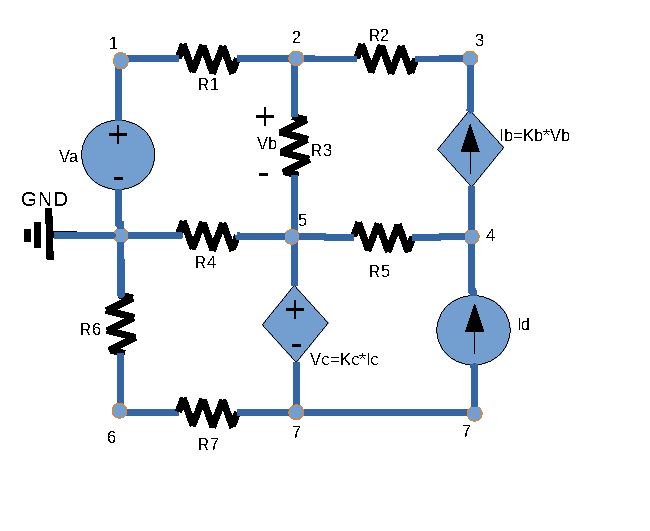
\includegraphics[width=0.8\linewidth]{t1_circuit.pdf}
\caption{Circuit with independent sources, dependent sources and resistors.}
\label{fig:t1_circuit}
\end{figure}

\begin{table}[h]
  \centering
  \begin{tabular}{|l|r|}
    \hline    
    {\bf Name} & {\bf Value [R, V, A and S]} \\ \hline
    R1 &  1030.3\\ \hline
R2 &  2030.8\\ \hline
R3 &  3094.4\\ \hline
R4 &  4087.1\\ \hline
R5 &  3005.2\\ \hline
R6 &  2031.1\\ \hline
R7 &  1047.6\\ \hline
Va &  5.0102\\ \hline
Id &  0.0010264\\ \hline
Kb &  0.0072761\\ \hline
Kc &  8137.0\\ \hline

  \end{tabular}
  \caption{Input values of Resistors, Voltage Source, Current Source and constants Kb and Kc.}
  \label{tab:input_values}
\end{table}


